% !TEX root = main.tex

\section{Symbolic Execution Engines}
\label{se:executors}

In this section we describe some important principles for the design of symbolic executors and crucial tradeoffs that arise in their implementation. Moving from the concepts of concrete and symbolic runs, we also introduce the idea of {\em concolic} execution.

\subsection{Mixing Symbolic and Concrete Execution}
\label{ss:concrete-concolic-symbolic}

\begin{figure}[t]
\centering

\includegraphics[width=0.35\columnwidth]{images/concrete-abstract.eps} 
\caption{Concrete and abstract execution machine models.}
\label{fig:concrete-symbolic}
\end{figure}

%%% 
%1) Main reasons why is hard to make symbolic execution to work in practice: 
%
%(a) Effects of any piece of code inside a program have to be handled by the engine. This requires a lot of effort since large applications are commonly built on top of very complex software stacks that are implemented in many different languages. Moreover, evaluating the effects of the interactions with the environment can be quite challenging. Section X discuss in detail how this has been done in practice.
%
%(b) SMT solvers have improved significantly during the last decades but they still can have issues when dealing with non-linear constraints. Querying the solver for each branch inside a path can be very time and memory consuming. Moreover, it could happen that some queries cannot be solved due to their constraint complexity, leaving the symbolic engine with no clear choice of how to proceed the exploration.
%
%2) An approach that have been proposed in literature that has significantly improved the applicability of symbolic execution is what is known as concolic execution. This is a combination of concrete execution and symbolic execution. The main idea is to start [...]
%
%3) Although the benefits given by concolic execution are quite evident in practice, there are disadvantages as well. Concretization drives the engine towards a specific path of a program. For any uninterpreted piece of code in the path, the engine is not able to understand how its side effects can be altered in order to exhibit different behaviors. As a first consequence, the engine may miss many interesting paths of the program, increasing the number of false negatives. Another critical consequence is known as path divergence. Whenever some piace of code is only executed concretely, then crucial side effects over the symbolic state may not be properly tracked an engine. This could result in imprecise path constraints, which in turn can lead the symbolic engine to generate new concrete inputs that do not actually follow the predicted path in the program. At the end, a concolic engine can waste quite a lot of resources due path divergence, resulting in reduced effectiveness.
%%%

As shown in the warm-up example (Section~\ref{symbolic-execution-example}), a symbolic execution of a program can generate -- in theory -- all possible control flow paths that the program could take during its concrete executions on specific inputs. While modeling all possible runs allows for very interesting analyses, it is typically unfeasible in practice, especially on real-world software. %, for a variety of reasons. 
%
\mytempedit{
Indeed, complex applications are often built on top of very sophisticated software stacks. Implementing a symbolic execution engine able to statically analyze the whole stack can be rather challenging given the difficulty in accurately evaluating any possible side effect during execution. Several problems arise in this context, which can hardly be faced following the purely symbolic approach of Section~\ref{symbolic-execution-example}:

\begin{enumerate}
\item\label{it:library-call-issue} Exhaustive exploration of external library calls may lead to an exponential explosion of states, preventing the analysis from reaching interesting code portions. %The problem is exacerbated by any interactions with the environment (files, network, etc.) made in the library.

\item\label{it:third-party-issue} Calls to external {\em third-party components} may not be traceable by the executor.

\item\label{it:smt-solver-issue} Symbolic engines continuously invoke {\em SMT solvers} during the analysis. The time spent in constraint solving is one of the main performance barriers for an engine, and programs may yield constraints that even powerful solvers cannot handle well.
%The time spent in constraint solving is one of the main performance barriers for symbolic engines, and a program may yields constraints (e.g., involving non-linear arithmetic) that even powerful SMT solvers cannot handle well.

%Although powerful SMT solvers are currently available, the time spent in constraint solving is still one of the main performance barriers for symbolic engines. It may also happen that the program yields constraints that the solver cannot handle well (e.g., non-linear constraints). %, in spite of the fact that symbolic executors often use more than one solver in order to support as many decidable logical fragments as possible.

%\item\label{it:smt-solver-issue} As observed in Section~\ref{se:intro}, symbolic engines are clients of {\em SMT solvers}, which are continuously invoked during the analysis. Although powerful SMT solvers are currently available, the time spent in constraint solving is still one of the main performance barriers for symbolic engines. It may also happen that the program yields constraints that the solver cannot handle well (e.g., non-linear constraints). %, in spite of the fact that symbolic executors often use more than one solver in order to support as many decidable logical fragments as possible.

%\item\label{it:symbolic-performance-issue} Due to abstract operations on symbolic expressions, symbolic execution tends to be intrinsically slower than concrete execution. %, posing a higher computational burden on the execution engine.

\end{enumerate}

\noindent A fundamental idea to cope with the aforementioned issues and to make symbolic execution feasible in practice is to mix concrete and symbolic execution: this is dubbed {\em concolic execution}, where the term concolic is a portmanteau of the words ``concrete'' and ``symbolic'' (Figure~\ref{fig:concrete-symbolic}). \mynote{fwd refs for 1, 2, 3?}
This general principle has been explored along different angles, discussed in the remainder of this section. %We discuss advantages and disadvantages of the different approaches, deferring an additional discussion of issue~(\ref{it:smt-solver-issue}) to Section~\ref{se:constraint-solving}.

%issues (\ref{it:library-call-issue}), (\ref{it:third-party-issue}), and (\ref{it:smt-solver-issue})
\myparagraph{Dynamic Symbolic Execution} One popular concolic execution approach, known as {\em dynamic symbolic execution} or {\em dynamic test generation}~\cite{DART-PLDI05}, is to have concrete execution drive symbolic execution. This technique can be very effective in mitigating the issues above. In addition to the symbolic store and the path constraints, the execution engine maintains a concrete store $\sigma_c$. After choosing an arbitrary input to begin with, it executes the program both concretely and symbolically by simultaneously updating the two stores and the path constraints. Whenever the concrete execution takes a branch, the symbolic execution is directed toward the same branch and the constraints extracted from the branch condition are added to the current set of path constraints. In short, the symbolic execution is driven by a specific concrete execution. As a consequence, the symbolic engine does not need to invoke the constraint solver to decide whether a branch condition is (un)satisfiable: this is directly tested by the concrete execution. In order to explore different paths, the path conditions given by one or more branches can be negated and the SMT solver invoked to find a satisfying assignment for the new constraints, i.e., to generate a new input. This strategy can be repeated as much as needed to achieve the desired coverage. 
}

\vspace{-2pt} 
\boxedexample{
Consider the C function in Figure~\ref{fig:example-1} and suppose to choose $a = 1$ and $b = 1$ as input parameters. Under these conditions, the concrete execution takes path $A\leadsto B\leadsto C\leadsto E\leadsto G$ in the symbolic tree of Figure~\ref{fig:example-symbolic-execution}. Besides the symbolic stores shown in Figure~\ref{fig:example-symbolic-execution}, the concrete stores maintained in the traversed states are the following:
  \begin{enumerate}
  
  \item[]$-$~~$\sigma_c=\{a\mapsto 1,~b\mapsto 1\}$ in state $A$;
  \item[]$-$~~$\sigma_c=\{a\mapsto 1,~b\mapsto 1,~x\mapsto 1,~y\mapsto 0\}$ in states $B$ and $C$;
  \item[]$-$~~$\sigma_c=\{a\mapsto 1,~b\mapsto 1,~x\mapsto 1,~y\mapsto 4\}$ in states $E$ and $G$.
  
  \end{enumerate}  
%Stores and path constraints maintained by the concolic run are shown in Figure~\ref{fig:example-concolic-execution}. 
After checking that the \texttt{assert} conditions at line 8 succeed, we can generate a new control flow path by negating the last path constraint, i.e., $\alpha_b\neq 0$. The solver at this point would generate a new input that satisfies the constraints $\alpha_a\neq 0\,\wedge\, \alpha_b=0$ (for instance $a = 1$ and $b = 0$) and the execution would continue in a similar way along the path $A\leadsto B\leadsto C\leadsto E\leadsto F$. %
}

%\mytempedit{First, as extensively discussed in Section~\ref{se:path-explosion}, the number of control flow paths to be generated and analyzed could be prohibitively large, due to branch instructions and loops. In the worst case, if the code contains an unbounded loop, symbolic execution could keep running forever, generating a potentially infinite number of paths (we refer to Section~\ref{se:path-explosion} for an example).}

%Moreover, as observed in Section~\ref{se:intro}, symbolic engines are clients of SMT solvers, which are continuously invoked during the analysis. Although powerful SMT solvers are currently available, the time spent in constraint solving is still one of the main performance barriers for symbolic engines. It may also happen that the program yields constraints that the solver cannot handle well (e.g., non-linear constraints), in spite of the fact that symbolic executors often use more than one solver in order to support as many decidable logical fragments as possible.
%An SMT instance is a formula in first-order logic, where some function and predicate symbols have additional meaning. This meaning depends on the theory being used: for instance, with linear inequalities symbols with extra meaning include the integers, $+$, $-$, $x$, $\le$. Path constraints are typically expressed in a decidable logical fragment without quantifiers

%A standard approach to limit the resources (running time and space usage) required by the execution engine and to handle complex constraints is to mix concrete and symbolic execution: this is dubbed {\em concolic execution}, where the term concolic is a portmanteau of the words concrete and symbolic. The basic idea is to have the concrete execution drive the symbolic execution (see also Figure~\ref{fig:concrete-symbolic}). Besides the symbolic store and the path constraints, a concolic execution engine also maintains a concrete store $\sigma_c$. After choosing an arbitrary input to begin with, it executes the program both concretely and symbolically by simultaneously updating the two stores and the path constraints. In order to explore different paths, the path conditions given by one or more branches can be negated and the SMT solver invoked to find a satisfying assignment for the new constraints, i.e., to generate a new input.

%Traditional symbolic execution does not scale over large programs. Although search heuristics may help prioritize some interesting paths, symbolic execution may still proceed extremely slow. 
%\mynote{[D] path conditions starting from the last one?}

%\begin{figure}[t]
%  \centering
%  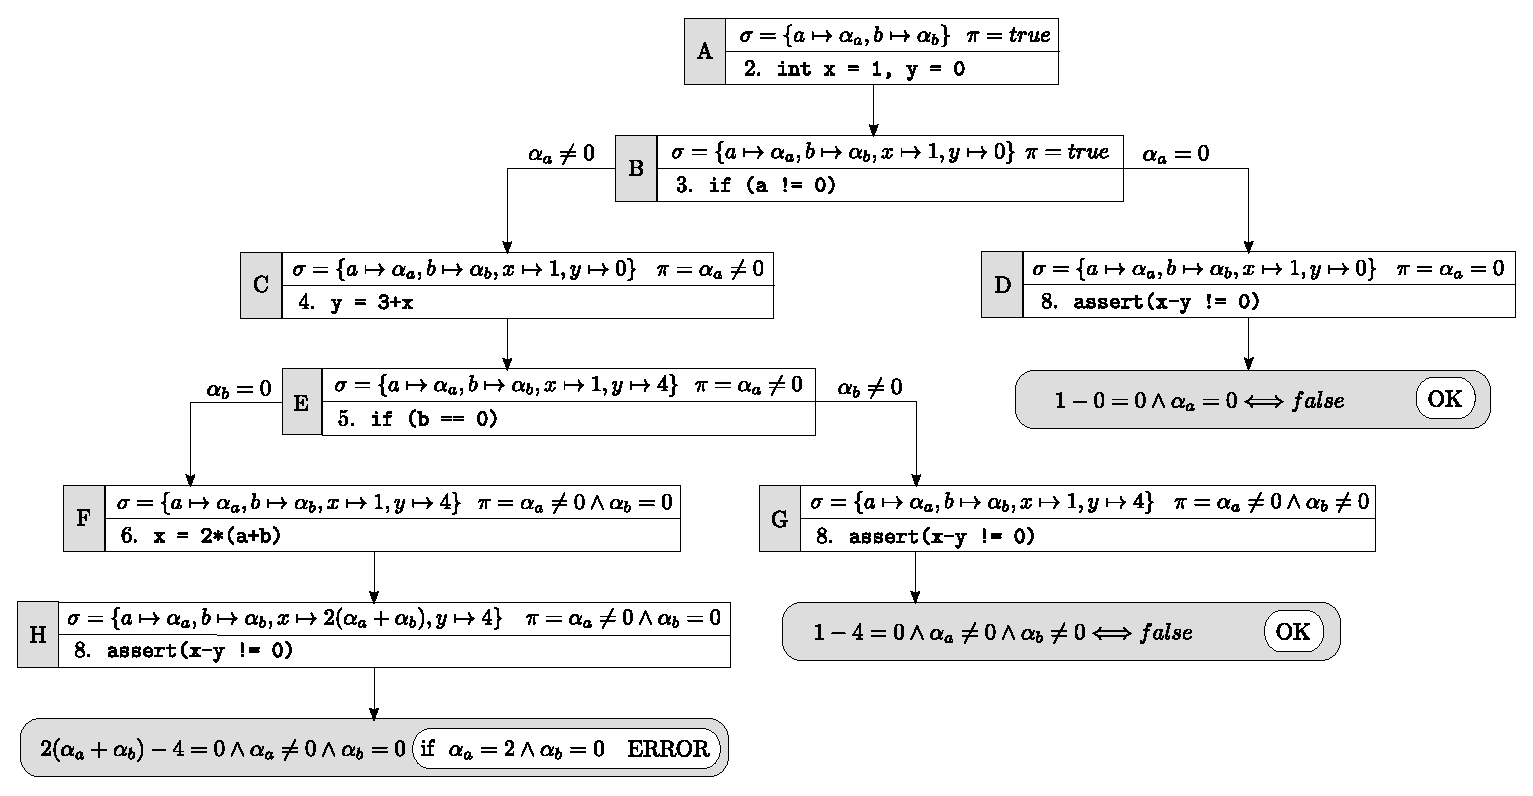
\includegraphics[width=1.0\columnwidth]{images/execution-tree.eps} 
%  \caption{TREE TO BE REPLACED. Concolic execution of function {\tt foobar} given in Figure~\ref{fig:example-1} starting with input $a = 1$ and $b = 1$. Besides the statement to be executed, the symbolic store $\sigma$, the path constraints $\pi$, execution states also show the concrete store $\sigma_c$. }
%%For the sake of presentation the conjunction of constraints is shown as a list of constraints. }
%  \label{fig:example-concolic-execution}
%\end{figure}

%\vspace{2mm}
%\noindent
%\fbox{%
%  \parbox{0.98\textwidth}{%
%  {\em Example.}  Consider the C function in Figure~\ref{fig:example-1} and suppose to choose $a = 1$ and $b = 1$ as input parameters. Under these conditions, the concrete execution takes path $A\leadsto B\leadsto C\leadsto E\leadsto G$ in the symbolic tree of Figure~\ref{fig:example-symbolic-execution}. Besides the symbolic stores shown in Figure~\ref{fig:example-symbolic-execution}, the concrete stores maintained in the traversed states are the following:
%  \begin{enumerate}
%  
%  \item[]$-$~~$\sigma_c=\{a\mapsto 1,~b\mapsto 1\}$ in state $A$;
%  \item[]$-$~~$\sigma_c=\{a\mapsto 1,~b\mapsto 1,~x\mapsto 1,~y\mapsto 0\}$ in states $B$ and $C$;
%  \item[]$-$~~$\sigma_c=\{a\mapsto 1,~b\mapsto 1,~x\mapsto 1,~y\mapsto 4\}$ in states $E$ and $G$.
%  
%  \end{enumerate}  
%%Stores and path constraints maintained by the concolic run are shown in Figure~\ref{fig:example-concolic-execution}. 
%After checking that the \texttt{assert} conditions at line 8 succeed, we can generate a new control flow path by negating the last path constraint, i.e., $\alpha_b\neq 0$. The solver at this point would generate a new input that satisfies the constraints $\alpha_a\neq 0\,\wedge\, \alpha_b=0$ (for instance $a = 1$ and $b = 0$) and the execution would continue in a similar way along the path $A\leadsto B\leadsto C\leadsto E\leadsto F$. }%
%}

\vspace{-2pt}  % TODO was +2mm
\mytempedit{
\noindent Although dynamic symbolic execution uses concrete inputs to drive the symbolic execution toward a specific path, it still needs to pick a branch to negate whenever a new path has to be explored. Notice also that each concrete execution may add new branches that will have to be visited. Since the set of non-taken branches across all performed concrete executions can be very large, adopting effective search heuristics (Section~\ref{ss:heuristics}) can play a crucial role. For instance, {\sc DART}~\cite{DART-PLDI05} chooses the next branch to negate using a depth-first strategy. Additional strategies for picking the next branch to negate have been presented in literature. For instance, the {\em generational search} algorithm discussed in {\sc SAGE}~\cite{SAGE-NDSS08} systematically yet partially explores the state space, maximizing the number of new tests generated while also avoiding redundancies in the search. This is achieved by negating constraints following a specific order and by limiting the backtracking of the search algorithm. Since the state space is only partially explored, the initial input plays a crucial role in the effectiveness of the overall approach.  The importance of the first input is similar to what happens in traditional {\em black-box fuzzing} and, for this reason, symbolic engines such as {\sc SAGE} are often referred to as {\em white-box fuzzers}.

The symbolic information maintained during a concrete run can be exploited by the execution engine, for instance, to obtain new inputs and explore new control flow paths. The next example shows how dynamic symbolic execution \mynote{[D] deals with?} can handle invocations to external code that is not symbolically tracked by the concolic engine.
%However, our previous example has not motivated in practice the two main benefits given by concolic execution: (a) use of the concolic store to help a SMT solver to efficiently handle non-linear constraints, (b) symbolic execution of a piece of code that contains invocations to external code that is not symbolically tracked by the concolic engine. While the first benefit will be better explained in Section~\ref{se:constraint-solving}, we now use the next example to explore the second benefit, pinpointing also some critical disadvantages that come with it. 
}

\vspace{-2pt}
\mytempedit{
\boxedexample{
Consider function {\tt foo} in Figure~\ref{fig:example-concolic-problems}a and suppose that {\tt bar} is not symbolically tracked by the concolic engine (e.g., it could be provided by a third-party component, written in a different language, or analyzed following a black-box approach). Assuming that $x = 1$ and $y = 2$ are randomly chosen as the initial input parameters, the concolic engine executes {\tt bar} (which returns $a = 0$) and skips the branch that would trigger the error statement. At the same time, the symbolic execution tracks the path constraint $\alpha_y \geq 0$ inside function {\tt foo}. Notice that branch conditions in function {\tt bar} are not known to the engine. To explore the alternative path, the engine negates the path constraint of the branch in {\tt foo}, generating inputs, such as $x = 1$ and $y = -4$, that actually drive the concrete execution to the alternative path. With this approach, the engine can explore both paths in {\tt foo} even if {\tt bar} is not symbolically tracked. 

A variant of the previous code is shown in Figure~\ref{fig:example-concolic-problems}b, where function {\tt qux} -- differently from {\tt foo} -- takes a single input parameter but checks the result of {\tt bar} in the branch condition. Although the engine can track the path constraint in the branch condition tested inside {\tt qux}, there is not guarantee than an input able to drive the execution toward the alternative path is generated: the relationship between $a$ and $x$ is not known to the concolic engine, as {\tt bar} is not symbolically tracked. In this case, the engine could re-run the code using a different random input, but in the end it could fail to explore one interesting path in {\tt foo}. 

A related issue is presented by Figure~\ref{fig:example-concolic-problems}c. Function {\tt baz} invokes the external function {\tt abs}, which simply computes the absolute value of a number. Choosing $x = 1$ as the initial concrete value, the concrete execution does not trigger the error statement, but the concolic engine tracks the path constraint $\alpha_x \geq 0$ due to the branch in {\tt baz}, trying to generate a new input by negating it. However the new input, e.g., $x = -1$, does not trigger the error statement due to the (untracked) side effects of {\tt abs}. In this case, after generating a new input the engine detects a {\em path divergence}: a concrete execution that does not follow the predicted path. Interestingly, in this example no input could actually trigger the error, but the engine is not able to detect this property.
}
}

\begin{figure*}[t]
  %\vspace{-3mm}
  %\centering
  \begin{subfigure}[t]{.33\textwidth}
    \begin{lstlisting}[basicstyle=\ttfamily\scriptsize]
void foo(int x, int y) {
   int a = bar(x);
   if (y < 0) ERROR;
} 
\end{lstlisting}
%int bar(int z) {
%   if (z == 23) return 1;
%   return 0;
%}
    \vspace{-4mm}
    \caption{}
  \end{subfigure}%
  %
  %\hspace{-2mm}
  %
  \begin{subfigure}[t]{.33\textwidth}
    %\vspace{5mm}
    \begin{lstlisting}[basicstyle=\ttfamily\scriptsize]
void qux(int x) {
   int a = bar(x);
   if (a > 0) ERROR;
} 
\end{lstlisting}
%int bar(int z) {
%   if (z == 23) return 1;
%   return 0;
%}
    \vspace{-4mm}
    \caption{}
  \end{subfigure}%
  %
  %\hspace{-2mm}
  %
  \begin{subfigure}[t]{.33\textwidth}
    %\vspace{5mm}
    \begin{lstlisting}[basicstyle=\ttfamily\scriptsize]
void baz(int x) {
   abs(&x);
   if (x < 0) ERROR;
}   
\end{lstlisting}
%void abs(int * z) {
%   if (*z < 0) *z = -(*z);
%}
    \vspace{-4mm}
    \caption{}
  \end{subfigure}%

  \vspace{-2mm}
  \caption{Concolic execution: (a) testing of function {\tt foo} even when {\tt bar} cannot be symbolically tracked by an engine, (b) example of false negative, and (c) example of a path divergence, where \texttt{abs} drops the sign of the integer at \texttt{\&x}.
   %(b) Example of a missed path: assuming that function {\tt bar} is not symbolically tracked, then it is unlikely that the engine will be able to generate an input that trigger execution of function {\tt error} inside function {\tt qux}. (c) Example of a path divergence: assuming that function {\tt abs} is not tracked, then the concolic engine may try to generate fruitlessly an input able to trigger execution of function {\tt error} in function {\tt baz}.
   }
  \label{fig:example-concolic-problems}
  \vspace{-3mm}
\end{figure*}

\vspace{-2pt} 
\mytempedit{
\noindent 
%Using concolic execution, many symbolic frameworks have been able to scale their analysis over large and complex applications. 
As shown by the example, false negatives (i.e., missed paths) and path divergences are notable downsides of dynamic symbolic execution. Dynamic symbolic execution trades soundness for performance and implementation effort: false negatives are possible, because some program executions -- and therefore possible erroneous behaviors -- may be missed, leading to a {\em complete}, but {\em under-approximate} form of program analysis. Path divergences have been extensively observed in literature: for instance,~\cite{SAGE-NDSS08} has reported rates over $60\%$. \cite{CLH-SCN15} has performed an empirical study of path divergences, analyzing the main patterns that contribute to this phenomenon. External calls, exceptions, type casts, and symbolic pointers were pinpointed as critical aspects during concolic execution that must be carefully handled by an engine to reduce the number of path divergences.
%Section~\ref{se:environment-thirdparty} will present some ideas (e.g., {\em selective symbolic execution}) that can help reduce the number of false negatives. 
}
%\mytempedit{
%To mitigate the problem of false negatives, several works have exploited variants of concolic execution or different ways of mixing concrete and symbolic runs. \cite{DBF-ISSTA16} presents a framework for the specification of mixed concrete/symbolic policies, allowing for a better understanding of their impact and trade-offs in terms of correctness, completeness and efficiency of the approach.} 

\myparagraph{Selective Symbolic Execution}
\mytempedit{{\sc \stwoe}~\cite{CKC-TOCS12} takes a different approach to mix symbolic and concrete execution based on the observation that one might want to explore only some components of a software stack in full, not caring about others. {\em Selective symbolic execution} carefully interleaves concrete and symbolic execution, while keeping the overall exploration meaningful.
%{\em Selective symbolic execution} carefully interleaves concrete executions of functions with fully symbolic phases, while keeping the exploration meaningful.

Suppose a function A calls a function B and the execution mode changes at the call site. Two scenarios arise:
(1) {\em From concrete to symbolic and back}: the arguments of B are made symbolic and B is explored symbolically. B is also executed concretely and its concrete result is returned to A. After that, A resumes concretely. 
(2) {\em From symbolic to concrete and back}: the arguments of B are concretized, B is executed concretely, and execution resumes symbolically in A. This may impact both soundness and completeness of the analysis: (i) {\em completeness}: to make sure that symbolic execution skips any paths that would not be realizable due to the performed concretization, {\sc \stwoe} collects constraints that keep track of how arguments are concretized, what side effects are made by B, and what returned value it produces. (ii) {\em Soundness}: concretization may cause missed branches after A is resumed. To remedy this, the collected constraints are marked as {\em soft}: whenever a branch after returning to A is made inoperative by a soft constraint, the execution backtracks and a different choice of arguments for B is attempted. To guide re-concretization of B's arguments, {\sc \stwoe} also collects the branch conditions during the concrete execution of B, and chooses the concrete values so that they enable a different concrete execution path in B.

%Going from the concrete to the symbolic domain is easy: the called function is executed both concretely and symbolically, with the result from the former simply returned to the concrete domain, while symbolic execution explores the component of interest in full by turning the arguments for the call into purely symbolic ones.

%Going instead from the symbolic to the concrete domain, the arguments for a call are concretized and added to the path constraints, as the return value and any possible side effects are a consequence of the values chosen for the arguments. This may result in missing future paths because of the constraints over the arguments values or the return value and side effects. The engine marks such constraints as {\em soft}: whenever a branch in the symbolic domain is made inoperative by a soft constraint, the execution backtracks and a different choice of arguments is attempted, possibly leveraging branch conditions tracked during the concrete execution.

%\mynote{I: inglese non fluido. and side effects a che si riferisce? Si intende because of side effects? Girare frase (prima side effects poi constraints)?}  

%The concrete-symbolic boundary traversal is ruled by an {\em execution consistency model} that balances path over- and under-approximation (i.e., false negatives/positives) with scalability. {\sc \stwoe} offers six models targeting different use cases (e.g., systematic testing, reverse engineering, analysis of cryptographic code with hard-to-solve constraints). 

%A transition from the symbolic domain is more complicated:

%Executions within the symbolic and concrete domains are dubbed multi-path and single-path, respectively.
}

%%% v0
%\myparagraph{Selective Symbolic Execution} \mytempedit{{\sc \stwoe}~\cite{CKC-TOCS12} takes a different approach to issues (\ref{it:library-call-issue}), (\ref{it:third-party-issue}), and (\ref{it:smt-solver-issue}), by interleaving portions of code that are concretely run with fully symbolic phases.} The interleaving must be done carefully in order to preserve the meaningfulness of the whole exploration. When an argument $x$ for a function call to be concretized is symbolic, the engine converts it to some concrete value in order to perform the call, which is equivalent to corseting the exploration to a single path in the callee. When the call returns and the symbolic phase resumes, the concrete value for $x$ becomes part of the path constraints for the remainder of the exploration. However, a large number of paths may be then excluded. {\sc \stwoe} presents a systematic approach to consistently cross the symbolic/concrete boundary in both directions: it describes a strategy to deal with constraints introduced on symbolic values as a consequence of concretization, and introduces a number of consistency models -- where a state is {\em consistent} when there exists a feasible path to it from the initial state -- which suit different analyses. Constraints that are updated to account for concrete values are marked as {\em soft}. Whenever a branch is made inoperative by such a constraint in the symbolic territory, execution goes back and picks a value for the concrete call that would enable that branch. %\mytempedit{Similarly to dynamic symbolic execution, this technique may incur in false negatives due to concretization.}

%Other techniques that could help reduce false negative will be later discussed in Section~\ref{se:constraint-solving}.

%\myparagraph{Execution-Generated Testing}\mynote{Is \cite{DBF-ISSTA16} crucial?} \mytempedit{A common concolic approach used for mitigating issues (\ref{it:smt-solver-issue}) and (\ref{it:symbolic-performance-issue}) lets the symbolic engine always execute concretely the operations that involve only concrete values. This idea, adopted, e.g., by {\sc KLEE}~\cite{KLEE-OSDI08}, {\sc EXE}~\cite{EXE-CCS06}, and~\cite{CS-CACM13}, can substantially speed up the computation and make it possible to reason even over complex (e.g., non-linear) operations if they involve only concrete values. We defer to Section~\ref{se:constraint-solving} an additional discussion of how concolic execution can help to cope with issue~(\ref{it:smt-solver-issue}). }

%Throughout this article, we will see other uses of concretization (see, e.g., Section~\ref{memory-model} and Section~\ref{se:constraint-solving})  and of concolic execution (see Section~\ref{se:path-explosion}).

% add something...


%\myparagraph{Dynamic Test Generation} 


%\mynote{Add paper on hybrid concolic testing}In particular,

%%%%%%%%%%%%%%%%%%%%%%%%%%%%%%%%%%%%%%%%%%%%%%%%%%%%%%%%%%%%%%%%%%%%%%%%%%%%%%%%%%%%
% Old sections about concolid execution and dynamic symbolic execution
%%%%%%%%%%%%%%%%%%%%%%%%%%%%%%%%%%%%%%%%%%%%%%%%%%%%%%%%%%%%%%%%%%%%%%%%%%%%%%%%%%%%

% \subsection{Concrete, Symbolic, and Concolic Execution}
% \label{ss:concrete-concolic-symbolic}

% As shown in the warm-up example (Section~\ref{symbolic-execution-example}), a symbolic execution of a program can generate -- in theory -- all possible control flow paths that the program could take during its concrete executions on specific inputs. While modeling all possible runs allows for very interesting analyses, it is typically unfeasible in practice, especially on real-world software, for a variety of reasons.

% \mytempedit{First, as extensively discussed in Section~\ref{se:path-explosion}, the number of control flow paths to be generated and analyzed could be prohibitively large, due to branch instructions and loops. In the worst case, if the code contains an unbounded loop, symbolic execution could keep running forever, generating a potentially infinite number of paths (we refer to Section~\ref{se:path-explosion} for an example).}

% Moreover, as observed in Section~\ref{se:intro}, symbolic engines are clients of SMT solvers, which are continuously invoked during the analysis. Although powerful SMT solvers are currently available, the time spent in constraint solving is still one of the main performance barriers for symbolic engines. It may also happen that the program yields constraints that the solver cannot handle well (e.g., non-linear constraints), in spite of the fact that symbolic executors often use more than one solver in order to support as many decidable logical fragments as possible.
% %An SMT instance is a formula in first-order logic, where some function and predicate symbols have additional meaning. This meaning depends on the theory being used: for instance, with linear inequalities symbols with extra meaning include the integers, $+$, $-$, $x$, $\le$. Path constraints are typically expressed in a decidable logical fragment without quantifiers

% \begin{figure}[t]
% \centering
% 
\includegraphics[width=0.35\columnwidth]{images/concrete-abstract.eps} 
% \caption{Concrete and abstract execution machine models.}
% \label{fig:concrete-symbolic}
% \end{figure}

% A standard approach to limit the resources (running time and space usage) required by the execution engine and to handle complex constraints is to mix concrete and symbolic execution: this is dubbed {\em concolic execution}, where the term concolic is a portmanteau of the words concrete and symbolic. The basic idea is to have the concrete execution drive the symbolic execution (see also Figure~\ref{fig:concrete-symbolic}). Besides the symbolic store and the path constraints, a concolic execution engine also maintains a concrete store $\sigma_c$. After choosing an arbitrary input to begin with, it executes the program both concretely and symbolically by simultaneously updating the two stores and the path constraints. In order to explore different paths, the path conditions given by one or more branches can be negated and the SMT solver invoked to find a satisfying assignment for the new constraints, i.e., to generate a new input.

% %\mynote{[D] path conditions starting from the last one?}

% %\begin{figure}[t]
% %  \centering
% %  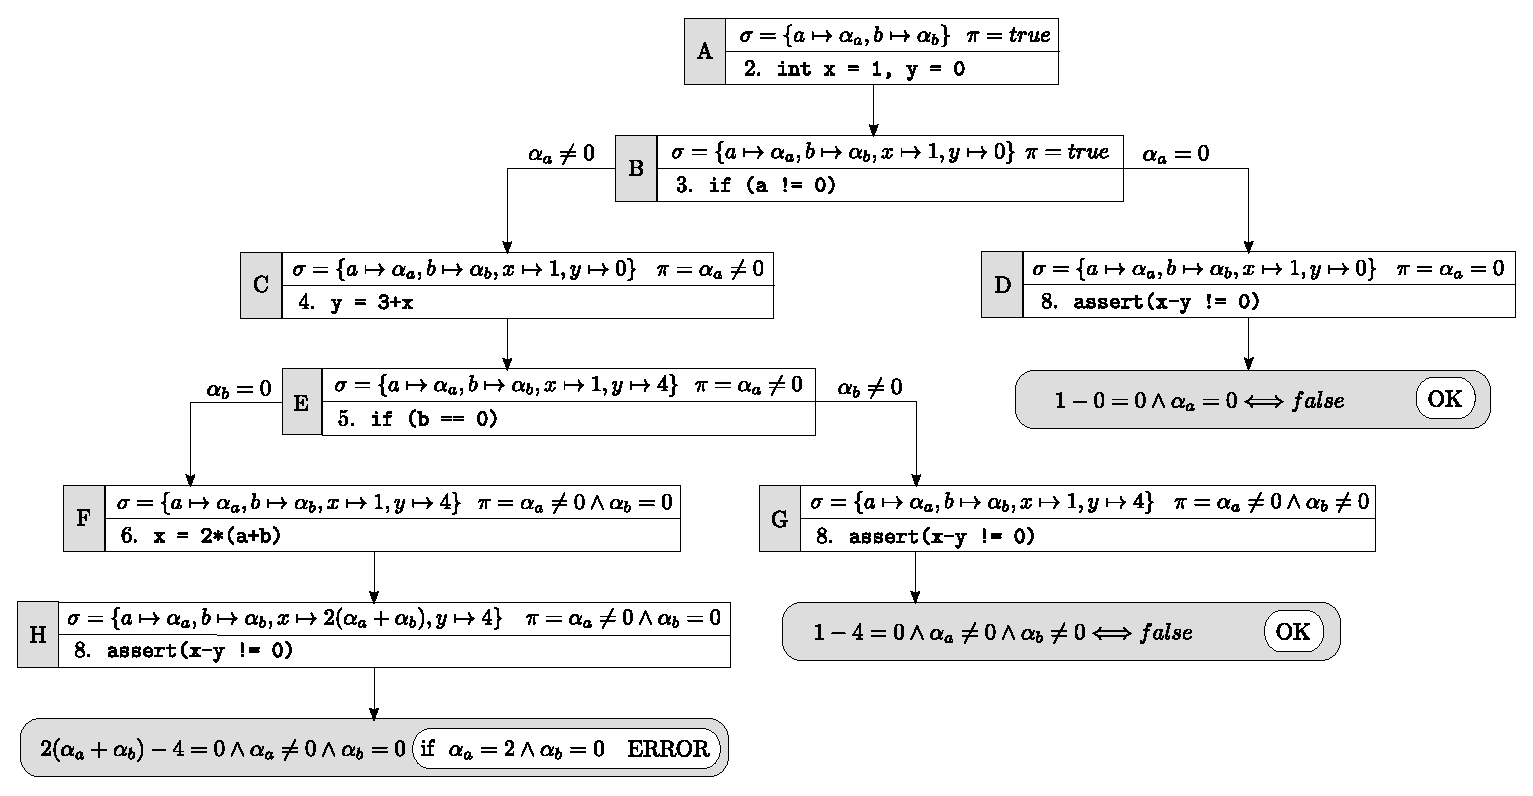
\includegraphics[width=1.0\columnwidth]{images/execution-tree.eps} 
% %  \caption{TREE TO BE REPLACED. Concolic execution of function {\tt foobar} given in Figure~\ref{fig:example-1} starting with input $a = 1$ and $b = 1$. Besides the statement to be executed, the symbolic store $\sigma$, the path constraints $\pi$, execution states also show the concrete store $\sigma_c$. }
% %%For the sake of presentation the conjunction of constraints is shown as a list of constraints. }
% %  \label{fig:example-concolic-execution}
% %\end{figure}

% \vspace{-2pt} % TODO
% \boxedexample{
% Consider the C function in Figure~\ref{fig:example-1} and suppose to choose $a = 1$ and $b = 1$ as input parameters. Under these conditions, the concrete execution takes path $A\leadsto B\leadsto C\leadsto E\leadsto G$ in the symbolic tree of Figure~\ref{fig:example-symbolic-execution}. Besides the symbolic stores shown in Figure~\ref{fig:example-symbolic-execution}, the concrete stores maintained in the traversed states are the following:
%   \begin{enumerate}
  
%   \item[]$-$~~$\sigma_c=\{a\mapsto 1,~b\mapsto 1\}$ in state $A$;
%   \item[]$-$~~$\sigma_c=\{a\mapsto 1,~b\mapsto 1,~x\mapsto 1,~y\mapsto 0\}$ in states $B$ and $C$;
%   \item[]$-$~~$\sigma_c=\{a\mapsto 1,~b\mapsto 1,~x\mapsto 1,~y\mapsto 4\}$ in states $E$ and $G$.
  
%   \end{enumerate}  
% %Stores and path constraints maintained by the concolic run are shown in Figure~\ref{fig:example-concolic-execution}. 
% After checking that the \texttt{assert} conditions at line 8 succeed, we can generate a new control flow path by negating the last path constraint, i.e., $\alpha_b\neq 0$. The solver at this point would generate a new input that satisfies the constraints $\alpha_a\neq 0\,\wedge\, \alpha_b=0$ (for instance $a = 1$ and $b = 0$) and the execution would continue in a similar way along the path $A\leadsto B\leadsto C\leadsto E\leadsto F$. %
% }

% %\vspace{2mm}
% %\noindent
% %\fbox{%
% %  \parbox{0.98\textwidth}{%
% %  {\em Example.}  Consider the C function in Figure~\ref{fig:example-1} and suppose to choose $a = 1$ and $b = 1$ as input parameters. Under these conditions, the concrete execution takes path $A\leadsto B\leadsto C\leadsto E\leadsto G$ in the symbolic tree of Figure~\ref{fig:example-symbolic-execution}. Besides the symbolic stores shown in Figure~\ref{fig:example-symbolic-execution}, the concrete stores maintained in the traversed states are the following:
% %  \begin{enumerate}
% %  
% %  \item[]$-$~~$\sigma_c=\{a\mapsto 1,~b\mapsto 1\}$ in state $A$;
% %  \item[]$-$~~$\sigma_c=\{a\mapsto 1,~b\mapsto 1,~x\mapsto 1,~y\mapsto 0\}$ in states $B$ and $C$;
% %  \item[]$-$~~$\sigma_c=\{a\mapsto 1,~b\mapsto 1,~x\mapsto 1,~y\mapsto 4\}$ in states $E$ and $G$.
% %  
% %  \end{enumerate}  
% %%Stores and path constraints maintained by the concolic run are shown in Figure~\ref{fig:example-concolic-execution}. 
% %After checking that the \texttt{assert} conditions at line 8 succeed, we can generate a new control flow path by negating the last path constraint, i.e., $\alpha_b\neq 0$. The solver at this point would generate a new input that satisfies the constraints $\alpha_a\neq 0\,\wedge\, \alpha_b=0$ (for instance $a = 1$ and $b = 0$) and the execution would continue in a similar way along the path $A\leadsto B\leadsto C\leadsto E\leadsto F$. }%
% %}

% %\vspace{2mm} % TODO rimosso
% \vspace{-2pt}  % TODO was +2mm
% \noindent As shown by the example, the symbolic information maintained during a concrete run can be exploited by the execution engine, for instance, to obtain new inputs and explore new control flow paths. We will further discuss this aspect in Section~\ref{ss:heuristics}. 

% It is worth noticing that concolic execution trades soundness for performance: false negatives are indeed possible, because some program executions -- and therefore possible erroneous behaviors -- may be missed. In the literature, this is also regarded as an {\em under-approximate} form of program analysis.

% % with fully symbolic phases, enabling program analysis across a full software stack without sacrificing scalability
% Many papers exploit variants of concolic execution or different ways of mixing concrete and symbolic runs. \mytempedit{\cite{DBF-ISSTA16} presents a framework for the specification of mixed concrete/symbolic policies, allowing for a better understanding of their impact and trade-offs in terms of correctness, completeness and efficiency of the approach.} For instance, in {\em execution-generated testing} (see, e.g., {\sc KLEE}~\cite{KLEE-OSDI08}, {\sc EXE}~\cite{EXE-CCS06}, and~\cite{CS-CACM13}, the symbolic engine always executes concretely the operations that involve only concrete values. This makes it possible to reason even over complex (e.g., non-linear) operations if they involve only concrete values. {\em Selective symbolic execution}~\cite{CKC-TOCS12} takes a different approach, by interleaving portions of code that are concretely run with fully symbolic phases. The interleaving must be done carefully in order to preserve the meaningfulness of the whole exploration. When an argument $x$ for a function call to concretize is symbolic, the engine should convert it to some concrete value in order to perform the call, which is equivalent to corseting the exploration to a single path in the callee. When the call returns and the symbolic phase resumes, the concrete value for $x$ becomes part of the path constraints for the remainder of the exploration. However, a large number of paths may be then excluded. {\sc \stwoe}~\cite{CKC-TOCS12} presents a systematic approach to consistently cross the symbolic/concrete boundary in both directions: it describes a strategy to deal with constraints introduced on symbolic values as a consequence of concretization, and introduces a number of consistency models -- where a state is {\em consistent} when there exists a feasible path to it from the initial state -- which suit different analyses. Constraints that are updated to account for concrete values are marked as {\em soft}. Whenever a branch is made inoperative by such a constraint in the symbolic territory, execution goes back and picks a value for the concrete call that would enable that branch. Throughout this article, we will see other uses of concretization (see, e.g., Section~\ref{memory-model} and Section~\ref{se:constraint-solving})  and of concolic execution (see Section~\ref{se:path-explosion}).

% %===================================================================================
% \subsection{Dynamic Symbolic Execution} 
% \label{ss:dynamic-symbolic-execution}

% %\myparagraph{Dynamic Test Generation} 
% Traditional symbolic execution does not scale over large programs. Although search heuristics may help prioritize some interesting paths, symbolic execution may still proceed extremely slow. Indeed, the engine must simulate any instruction in the program and heavily relies on the constraint solver in order to make any progress in the execution. {\em Dynamic test generation}, initially introduced in {\sc DART}~\cite{DART-PLDI05}, is a technique that can help symbolic execution scale to large programs. The main idea is to execute a program both concretely and symbolically. This kind of execution is often referred to as concolic execution (Section~\ref{ss:concrete-concolic-symbolic}). Initially, a random input is generated and a concrete execution is started. In parallel, a symbolic execution is also started. Whenever the concrete execution takes a branch, the symbolic execution is directed toward the same branch and the constraints extracted from the branch condition are added to the current set of path constraints. In other words, the symbolic execution is driven by a specific concrete execution. A consequence of this approach is that the symbolic engine does not need to invoke the constraint solver to decide whether a branch condition is (un)satisfiable, since this is directly tested by the concrete execution. Other paths of the program execution can be then explored by selecting a previously taken branch and negating its constraints. Using a constraint solver, the symbolic engine can generate a new (random) input that drives the concrete execution toward a new path. This strategy can be repeated as much as needed to achieve the desired coverage.

% \begin{figure}[t]
%   %\vspace{-3mm}
%   %\centering
%   \begin{subfigure}{.29\textwidth}
%     \vspace{5mm}
%     \begin{lstlisting}[basicstyle=\ttfamily\scriptsize]
% int bar(int x, int y) {
%    if (x < 5 && y >= 6) 
%       if (x > 1) return 1;
%       else return 2;
%    else return 3;
% }
%     \end{lstlisting}
%     \vspace{5mm}
%     \caption{}
%   \end{subfigure}%
%   \hspace{-2mm}
%   \begin{subfigure}{.37\textwidth}
%     \centering
%     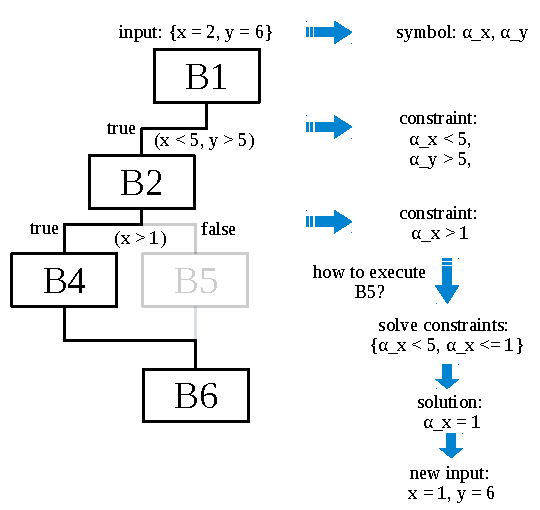
\includegraphics[width=1.0\columnwidth]{images/concolic-execution} 
%     %\label{fig:sub1}
%     \caption{}
%   \end{subfigure}%
%   \hspace{-2mm}
%   \begin{subfigure}{.33\textwidth}
%     \centering
%     \vspace{0.03mm}
%     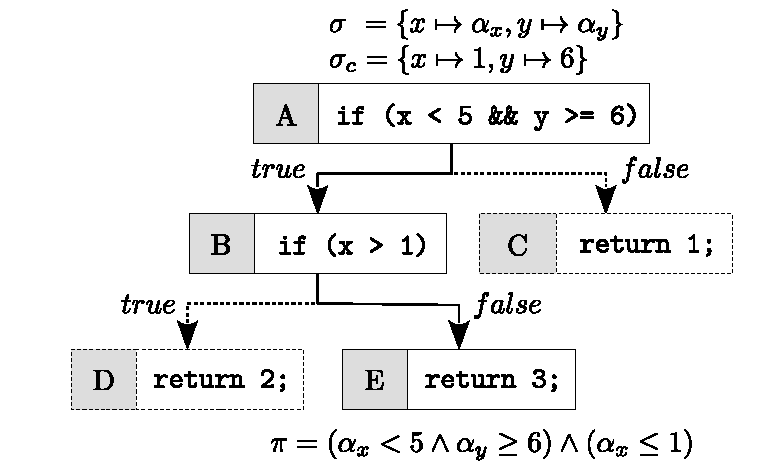
\includegraphics[width=1.1\columnwidth]{images/concolic-execution-2} 
%     %\label{fig:sub2}
%     %\vspace{0.0mm}
%     \caption{}
%   \end{subfigure}
%   \vspace{-2mm}
%   \caption{Dynamic test generation example. (a) Source code of function {\tt bar}. (b) Symbolic execution tree for the function {\tt bar}. Solid edges show the path taken by the concolic execution when {\tt x = 2} and {\tt y = 6}. These input values have been randomly chosen. (c) Concolic execution when {\tt x = 1} and {\tt y = 6}. These input values have been obtained using a constraint solver, after negating the path constraints of \iffullver{node B in the function {\tt bar}}{node B}.}
%   \label{fig:example-concrete-execution}
%   \vspace{-3mm}
% \end{figure}

% % pick the values {\tt x = 2} and {\tt y = 6}, respectively
% \vspace{-3pt} % TODO
% \boxedexample{ An example of dynamic test generation is shown in Figure~\ref{fig:example-concrete-execution}. Consider the function {\tt bar} (Figure~\ref{fig:example-concrete-execution}a) that takes two integer inputs {\tt x} and {\tt y}. To start a first concrete execution, a symbolic engine may initially randomly pick {\tt x = 2} and {\tt y = 6} as input values. The concrete execution induced by these inputs is presented in Figure~\ref{fig:example-concrete-execution}b: both the first and second branch condition (nodes $A$ and $B$) are satisfied, directing the execution toward the first {\tt return} statement (node $D$). Nodes $C$ and $E$ are skipped since their associated branch conditions are not met by the current input values. For instance, node $E$ is not executed since the condition $x > 1$ (node $B$) directs the path toward the node $D$. An engine that desires to symbolically execute a path containing the node $E$ must track the constraints during the concrete execution over {\tt x = 2} and {\tt y = 6} and then negate the branch condition $x > 1$. To generate a new input, the engine then invokes a solver over the constraints $\neg(\alpha_x > 1) \wedge (\alpha_x < 5 \wedge \alpha_y > 5)$, getting, e.g., {\tt x = 1} and {\tt y = 6} (Figure~\ref{fig:example-concrete-execution}c). Notice that since {\tt y} is not involved in the branch condition that is currently negated, the engine may reuse its value and include an additional constraint $\alpha_y = 6$. This optimization may drastically reduce the solving time required to obtain a solution from the constraint solver.}
% \vspace{-3pt} % TODO

% % that still need to be visited
% % what is done with
% \noindent Although dynamic test generation uses concrete inputs to drive the symbolic execution toward a specific path, it still needs to pick a branch to negate whenever a new path has to be explored. Notice also that each concrete execution may add new branches that will have to be visited. Since the set of non-taken branches across all the performed concrete executions can be very large, the search heuristics discussed in Section~\ref{ss:heuristics} still play a crucial role. For instance, {\sc DART}~\cite{DART-PLDI05} chooses the next branch to negate using a DFS strategy. Additional strategies for picking the next branch to negate have been presented in literature. For instance, the {\em generational search} algorithm discussed in {\sc SAGE}~\cite{SAGE-NDSS08} systematically yet partially explores the state space, maximizing the number of new tests generated while also avoiding redundancies in the search. This is achieved by negating constraints following a specific order and by limiting the backtracking of the search algorithm. Since the state space is only partially explored, the initial input plays a crucial role in the effectiveness of the overall approach.  The importance of the first input is similar to what happens in traditional {\em black-box fuzzing} and, for this reason, symbolic engines such as {\sc SAGE} are often referred as {\em white-box fuzzers}.

%===================================================================================
\subsection{Design Principles of Symbolic Executors}
\label{ss:principles}

A number %\mynote{[D] why MAYHEM?}  
of performance-related design principles that a symbolic execution engine should follow are  summarized in %{\sc Mayhem}
\cite{MAYHEM-SP12}. Most notably:
\begin{enumerate}
  \item {\em Progress}: the executor should be able to proceed for an arbitrarily long time without exceeding the given resources. Memory consumption can be especially critical, due to the potentially gargantuan number of distinct control flow paths.
  \item {\em Work repetition}: no execution work should be repeated, avoiding to restart a program several times from its very beginning in order to analyze different paths that might have a  common prefix.
  \item {\em Analysis reuse}: analysis results from previous runs should be reused as much as possible. In particular, costly invocations to the SMT solver on  previously solved path constraints should be avoided.
\end{enumerate}

\noindent Due to the large size of the execution state space to be analyzed, different symbolic engines have explored different tradeoffs between, e.g., running time and memory consumption, or performance and soundness/completeness of the analysis.

Symbolic executors that attempt to execute multiple paths simultaneously in a single run -- also called {\em online} -- clone the execution state at each input-dependent branch. Examples are given in {\sc KLEE}~\cite{KLEE-OSDI08}, {\sc AEG}~\cite{AEG-NDSS11}, {\sc \stwoe}~\cite{CKC-TOCS12}. These engines never re-execute previous instructions, thus avoiding work repetition. However, many active states need to be kept in memory and memory consumption can be large, possibly hindering progress. Effective techniques for reducing the memory footprint include {\em copy-on-write}, which tries to share as much as possible between different states~\cite{KLEE-OSDI08}. As another issue, executing multiple paths in parallel requires to ensure isolation between execution states, e.g., keeping different states of the OS by emulating the effects of system calls.

Reasoning about a single path at a time, as in concolic execution, is the approach taken by so-called {\em offline executors}, such as {\sc SAGE}~\cite{SAGE-NDSS08}. Running each path independently of the others results in low memory consumption with respect to online executors and in the capability of reusing immediately analysis results from previous runs. On the other side, work can be largely repeated, since each run usually restarts the execution of the program from the very beginning. In a typical implementation of offline executors, runs are concrete and require an input seed: the program is first executed concretely, a trace of instructions is recorded, and the recorded trace is then executed symbolically.

{\em Hybrid executors} such as {\sc Mayhem}~\cite{MAYHEM-SP12} attempt at balancing between speed and memory requirements: they start in online mode and generate checkpoints, rather than forking new executors, when memory usage or the number of concurrently active states reaches a threshold. Checkpoints maintain the symbolic execution state and replay information. When a checkpoint is picked for restoration, online exploration is resumed from a restored concrete state.
%: mixed approach. Start with an online approach, if needed switch to offline mode by doing checkpoints. A checkpoint contains the symbolic execution state and replay information. Concrete execution state is discarded since it can be quickly recovered at runtime by using one input generated by the solver before checkpointing.

%===================================================================================
\subsection{Path Selection}
\label{ss:heuristics}

\mytempedit{Since enumerating all paths of a program can be prohibitively expensive, in many software engineering activities related to testing and debugging the search is prioritized by looking at the most promising paths first. Among several strategies for selecting the next path to be explored, we now briefly overview some of the most effective ones. %in prior works.
}
%\subsubsection{Search Heuristics}
%\label{sss:search-heuristics}
%
% many prior works
%\myparagraph{Search Heuristics} 
We remark that path selection heuristics are often tailored to help the symbolic engine achieve specific goals (e.g., overflow detection). Finding a universally \mynote{I: universally optimal, ma e' fattibile?}  optimal strategy remains an open problem. %Table~\ref{tab:heuristics} provides a sample of prominent approaches. 

% "Common path selection heuristics" table moved to Appendix

{\em Depth-first search} (DFS), which expands a path as much as possible before backtracking to the deepest unexplored branch, and {\em breadth-first search} (BFS), which expands all paths in parallel, are the most common strategies. DFS is often adopted when memory usage is at a premium, but is hampered by paths containing loops and recursive calls. Hence,  in spite of the higher memory pressure and of the long time required to complete the exploration of specific paths, some tools resort to BFS, which allows the engine to quickly explore diverse paths  detecting interesting behaviors early. \iffullver{On the other hand, if the ultimate goal requires to fully terminate the exploration of one or more paths, BFS may take a very long time} Another popular strategy is {\em random path selection}, that has been refined in several variants. For instance, {\sc KLEE}~\cite{KLEE-OSDI08} assigns probabilities to paths based on their length and on the branch arity: it favors paths that have been explored fewer times, preventing starvation caused by loops and other path explosion factors.

% have instead presented
Several works, such as {\sc EXE}~\cite{EXE-CCS06}, {\sc KLEE}~\cite{KLEE-OSDI08}, {\sc Mayhem}~\cite{MAYHEM-SP12}, and {\sc \stwoe}~\cite{CKC-TOCS12}, have discussed heuristics aimed at maximizing code coverage. For instance, the {\em coverage optimize search} discussed in {\sc KLEE}~\cite{KLEE-OSDI08} computes for each state a weight, which is later used to randomly select states. The weight is obtained by considering how far the nearest uncovered instruction is, whether new code was recently covered by the state, and the state's call stack. Of a similar flavor is the heuristic proposed in~\cite{LZL-OOPSLA13}, called {\em subpath-guided search}, which attempts to explore {\it less traveled} parts of a program by selecting the subpath of the control flow graph that has been explored fewer times. This is achieved by maintaining a frequency distribution of explored subpaths, where a subpath is defined as a consecutive subsequence of length $n$ from a complete path. Interestingly, the value $n$ plays a crucial role with respect to the code coverage achieved by a symbolic engine using this heuristic and no specific value has been shown to be universally optimal. %
\mytempedit{
  Another interesting search strategy is the {\em shortest-distance symbolic execution} heuristic presented in~\cite{MPF-SAS11}. The work does not target coverage, but aims at identifying program inputs that trigger the execution of a specific point in a program. However, similarly to coverage-based strategies, it is based on a metric for evaluating the shortest distance to the target point. This is computed as the length of the shortest path in the inter-procedural control-flow graph, and paths with the shortest distance are prioritized by the engine. 
}

%Other search heuristics try to prioritize paths likely leading to states that are {\em interesting} according to some goal. For instance, the {\em buggy-path first} strategy in {\sc AEG}~\cite{AEG-NDSS11} picks paths whose past states have contained small but unexploitable bugs. The intuition is that if a path contains some small errors, it is likely that it has not been properly tested. There is thus a good chance that future states may contain interesting, and hopefully exploitable, bugs. Similarly, the {\em loop exhaustion} strategy discussed in {\sc AEG}~\cite{AEG-NDSS11} explores paths that visit loops. This approach is inspired by the practical observation that common programming mistakes in loops may lead to buffer overflows or other memory-related errors. In order to find exploitable bugs, {\sc Mayhem}~\cite{MAYHEM-SP12} instead gives priority to paths where symbolic memory accesses are identified or symbolic instruction pointers are detected. 

Other search heuristics try to prioritize paths likely leading to states that are {\em interesting} according to some goal. For instance, {\sc AEG}~\cite{AEG-NDSS11} introduces two such strategies. The {\em buggy-path first} strategy picks paths whose past states have contained small but unexploitable bugs. The intuition is that if a path contains some small errors, it is likely that it has not been properly tested. There is thus a good chance that future states may contain interesting, and hopefully exploitable, bugs. Similarly, the {\em loop exhaustion} strategy explores paths that visit loops. This approach is inspired by the practical observation that common programming mistakes in loops may lead to buffer overflows or other memory-related errors. In order to find exploitable bugs, {\sc Mayhem}~\cite{MAYHEM-SP12} instead gives priority to paths where memory accesses to symbolic addresses are identified or symbolic instruction pointers are detected. 

\mytempedit{\cite{ZCWDL15} proposes a novel method of dynamic symbolic execution to automatically find a program path satisfying a regular property, i.e., a property (such as file usage or memory safety) that can be represented by a Finite State Machine (FSM). Dynamic symbolic execution is guided by the FSM so that branches of an execution path that are most likely to satisfy the property are \mynote{[D] explored?} generated first. The approach exploits both static and dynamic analysis to compute the priority of a path to be selected for exploration: the states of the FSM that the current execution path has already reached are computed dynamically during the symbolic execution, while backward dataflow analysis is used to compute the future states statically. If the intersection of these two sets is non-empty, there is likely a path satisfying the property.
}

{\em Fitness functions} have been largely used in the context of search-based test generation~\cite{M-STVR04}. %\mynote{[D] Check and rephrase 2nd sentence}
A fitness function measures how close an explored path is to achieve the target test coverage. Several papers, e.g.,~\cite{XTD-DSN09,CS-CACM13}, have applied this idea in the context of symbolic execution. As an example,~\cite{XTD-DSN09} introduces {\em fitnex}, a strategy for concolic execution that prioritizes paths that are {\em closer} to take a specific branch. In more detail, given a branch condition of the form $|a - c| == 0$ and a \mynote{I: l'inglese (e il concetto) non e' molto chiaro, si puo' spiegare meglio?}  path that has reached the branch, {\em fitnex} computes a closeness equal to $|a - c|$ by leveraging the concrete values \iffullver{of the two}{of} variables $a$ and $c$ in that path. Similar fitness values can be computed for other kinds of branch conditions. The path with the lowest fitness value for a branch is selected by the symbolic engine. Paths that have not reached the branch yet get the worst-case fitness value. 

\mytempedit{Based on the observation that a large number of paths can be considered ``equivalent'' since the symbolic expressions describing the output are the same, \cite{QNR13} proposes a path partitioning approach where two program paths are placed in the same partition if they have the same relevant slice with respect to the program output. A relevant slice is the transitive closure of dynamic data and control dependencies as well as potential dependencies, which capture statements that affect the output by not getting executed. Paths are partitioned on-the-fly during their exploration, computing a concise semantic signature for a program, which describes all the different symbolic expressions that the output can assume along different paths.}

% \mytempedit{
% Different works~\cite{DA-ASE14,MPF-SAS11} aim at identifying program inputs that trigger the execution of a specific target point in a program.
% %: this goal is often referred as the {\em line reachability problem}. 
% For instance,~\cite{MPF-SAS11} presents different strategies to achieve this goal. Similarly to coverage-based heuristics, the {\em shortest-distance symbolic execution} strategy (SDSE) exploits a metric for evaluating the shortest distance to a target point (instead of any uncovered line in the code). This metric is defined as the length of the shortest path in the inter-procedural control-flow graph (ICFG). Paths with the shortest distance are prioritized by the engine. 
% %
% On the other hand, the {\em call-chain backward symbolic execution} strategy (CCBSE) works very differently. It starts by determining a valid path in the function where the target line is located. When a path is found, the strategy backwards to one of the possible callers of the function that contains the target point and tries to reconstruct a valid path from the entry point of the caller to the target point. This process is recursively repeated until a valid path from the main function of the program has been reconstructed. The main difference with respect to symbolic backward execution (see Section~\ref{se:executors}) is that, although CCBSE follows the call-chain backwards from the target point, inside each function the exploration is done as in traditional forward symbolic execution. Since both SDSE and CCBSE can behave poorly in some specific cases,~\cite{MPF-SAS11} has also proposed {\em Mix-CCBSE}, a combination of these two strategies that can perform very effectively in practice.
% }


%===================================================================================
%\subsection{Caching} 
%\label{ss:caching}

%Caching is a powerful technique to achieve time-space tradeoffs and is embodied in symbolic executors in different ways. Most prominently:

%\begin{itemize}[topsep=3pt] % TODO

%\item {\em Function caching.} A function $f$, and more in general any part of a program, may be called multiple times during an execution, either at the same calling context or at different ones. The traditional symbolic execution approach requires to symbolically execute $f$ at each call. \cite{G-POPL07} proposes a compositional approach that dynamically generates {\em function summaries}, allowing the symbolic executor to effectively reuse prior discovered analysis results. A similar idea has been also proposed in~\cite{BCE-TACAS08}. The main intuition is that, if two program states differ only for some program values that are not read later, the executions generated by the two program states will produce the same side effects. Side effects of a portion of code can be therefore cached and possibly reused later. 

%Since the two techniques are almost equivalent, our discussion will follow~\cite{G-POPL07}. 
%\paragraph{Definition of function summaries} A function summary $\phi_f$ for a function $f$ is defined as a propositional logic formula. It can be computed by successive iterations and defined as a disjunction of formulas $\phi_w$ of the form $\phi_w = {pre}_w \wedge post_w$, where $w$ is a possible execution path of function $f$, $pre_w$ is a conjunction of constraints over the inputs of $f$, and $post_w$ is a conjunction of constraints over the outputs of $f$. Formally, $\phi_f = \bigvee \phi_w$.  
%
%\paragraph{Using function summaries} Whenever a function $f$ is called, the symbolic execution engine checks whether a summary $\phi_w$ of $f$ with $pre_w$ compliant with the current path constraints is available. If so, the post conditions $post_w$ are added to the current symbolic state. Otherwise, if no matching summary is found, a new function summary is computed.
%
%\paragraph{Computing function summaries} Function summaries can be computed dynamically: whenever there is an invocation of a function $f$, $pre_w$ is obtained from the current set of constraints over the input of $f$, while $post_w$ is given by tracking constraints over the \mynote{[D] no symbolic?}concolic\footnote{{\em [D] If this technique applies to concolic executors only we should say it upfront!}} execution of function $f$ over some concrete inputs that are compliant with $pre_w$. Notice that $pre_w$ defines an equivalence class of concrete executions that result in executions characterized by $post_w$. 
%
%\paragraph{Issues} If the symbolic execution engine cannot reason on one or more statements contained in a function $f$, then the generated summary cannot be \mynote{[D] blindly}blindly reused. For instance, consider a function that contains a call to an external function (e.g., a system call) or to a {\em complex} one (e.g., a hash function). In this scenario, even if a matching function summary is found, the related post conditions $post_w$ may not be valid since they have been generated over a concrete execution and thus cannot be generalized. % robust hash function

%\item {\em Loop summarization.} In order to avoid redundant executions of the same loop under the same program state, loop summaries can be computed and cached for later reuse, similarly to function summaries. We refer to Section~\ref{se:loops} for details on a loop summarization strategy proposed in~\cite{GL-ISSTA11}.

%\item {\em Constraint reuse.} In order to speed up constraint solving, different works support the reuse of constraint solutions based on semantic or syntactic equivalence of the constraints. Examples are given in {\sc EXE}~\cite{EXE-CCS06}, {\sc KLEE}~\cite{KLEE-OSDI08}, and~\cite{MEMO-ISSTA12,GREEN-FSE12}. We will further discuss this optimization in Section~\ref{se:constraint-solving}.

%\end{itemize}

\mytempedit{
\subsection{Symbolic Backward Execution}
\label{ss:backward}
% Symbolic backward execution (SBE)~\cite{CFS-PLDI09,DA-ASE14} is a variant of symbolic execution that proceeds its exploration backward from a target point of a program to an entry point of a program. In other words, the analysis is performed in the reversed direction with respect to a traditional (forward) symbolic execution.
Symbolic backward execution (SBE)~\cite{CFS-PLDI09,DA-ASE14} is a variant of symbolic execution in which the exploration proceeds from a target point to an entry point of a program. The analysis is thus performed in the reverse direction than in canonical (forward) symbolic execution. The main purpose of this approach is typically to identify a test input instance that can trigger the execution of a specific line of code (e.g., an {\tt assert} or {\tt throw} statement). %  
This can very useful for a developer when performing debugging or regression testing over a program.
As the exploration starts from the target, path constraints are collected along the branches met during the traversal. Multiple paths can be explored at a time by an SBE engine and, akin to forward symbolic execution, paths are periodically checked for feasibility. When a path condition is proven unsatisfiable, the engine discards the path and backtracks.
%SBE starts its exploration from a target point and steps backwards into the code, collecting the path constraints given by the branches that are met during the traversal. In general, multiple paths can be simultaneously explored by a SBE engine. Akin to forward symbolic execution, paths are periodically checked to verify their feasibility. Whenever a path condition is proven to be unsatisfiable, the engine discards the path and then backtracks. 


\cite{MPF-SAS11} discusses a variant of SBE dubbed {\em call-chain backward symbolic execution}~(CCBSE). The technique starts by determining a valid path in the function where the target line is located. When a path is found, the engine moves to one of the callers of the function that contains the target point and tries to reconstruct a valid path from the entry point of the caller to the target point. The process is recursively repeated until a valid path from the main function of the program has been reconstructed. The main difference with respect to the traditional SBE is that, although CCBSE follows the call-chain backwards from the target point, inside each function the exploration is done as in traditional symbolic execution.

%A variant of SBE has been discussed by~\cite{MPF-SAS11} with the {\em call-chain backward symbolic execution} strategy (CCBSE). This technique starts by determining a valid path in the function where the target line is located. When a path is found, the strategy backwards to one of the callers of the function that contains the target point and tries to reconstruct a valid path from the entry point of the caller to the target point. This process is recursively repeated until a valid path from the main function of the program has been reconstructed. The main difference with respect to the traditional SBE is that, although CCBSE follows the call-chain backwards from the target point, inside each function the exploration is done as in traditional symbolic execution.

A crucial requirement for the reversed exploration in SBE, as well as in CCBSE, is the availability of the inter-procedural control-flow graph which provides a whole-program control flow and makes it possible to determine the call sites for the functions that are involved in the exploration. Unfortunately, constructing such a graph can be quite challenging in practice\iffullver{ (see, e.g., the discussion about CFG reconstruction in Section~\ref{se:symbolic-binary}).}{\mynote{cite appendix or some paper?}.} Moreover, a function may have many possible call sites, making the exploration performed by a SBE still very expensive. On the other hand, some practical advantages can arise when the constraints are collected in the reverse direction. We will further discuss these benefits in Section~\ref{se:constraint-solving}.
}

% "Tools" moved to Appendix